\documentclass[border=3mm]{standalone}
\usepackage{ctex}
\usepackage{tikz}
\usetikzlibrary{positioning, arrows.meta, shapes.geometric, fit, backgrounds, calc}

\begin{document}
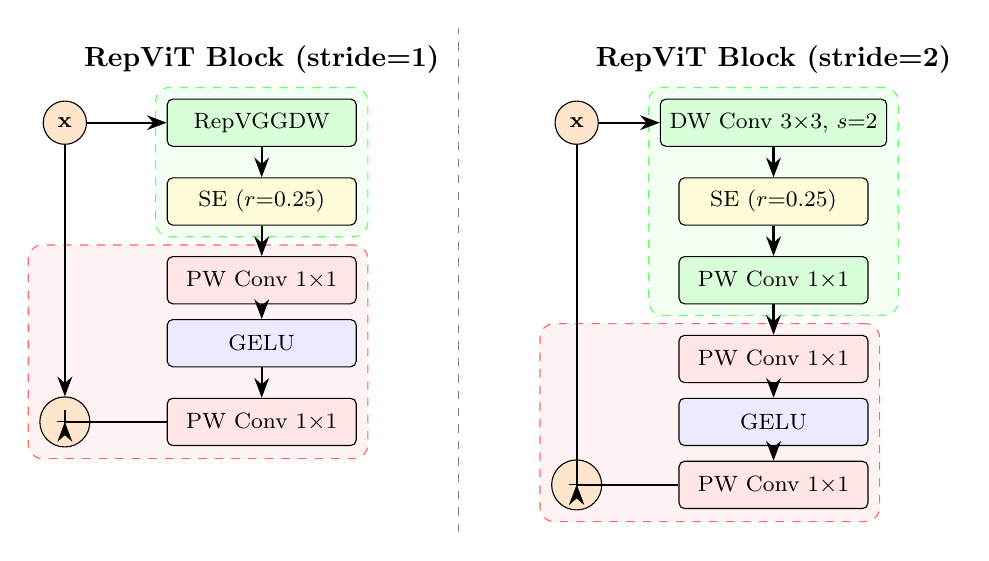
\begin{tikzpicture}[
    node distance=0.6cm and 0.8cm,
    block/.style={rectangle, draw, rounded corners=3pt, minimum width=2.8cm, minimum height=0.7cm, align=center, font=\small},
    op/.style={rectangle, draw, rounded corners=2pt, minimum width=2.4cm, minimum height=0.6cm, align=center, fill=blue!8, font=\footnotesize},
    data/.style={circle, draw, minimum size=0.5cm, fill=orange!20, font=\footnotesize},
    arrow/.style={-{Stealth[length=2.5mm]}, thick},
    dasharrow/.style={-{Stealth[length=2mm]}, thick, dashed, gray},
    label/.style={font=\footnotesize\itshape, text=gray},
]

% ====== stride=1 Block ======
\node[font=\normalsize\bfseries] at (0, 4.8) {RepViT Block (stride=1)};

\node[data] (x1) at (-2.5, 4) {$\mathbf{x}$};
\node[op, fill=green!15] (dw1) at (0, 4) {RepVGGDW};
\node[op, fill=yellow!15] (se1) at (0, 3.0) {SE ($r{=}0.25$)};
\node[op, fill=red!10] (pw1a) at (0, 2.0) {PW Conv $1{\times}1$};
\node[op] (gelu1) at (0, 1.2) {GELU};
\node[op, fill=red!10] (pw1b) at (0, 0.2) {PW Conv $1{\times}1$};
\node[data] (out1) at (-2.5, 0.2) {$+$};

\draw[arrow] (x1) -- (dw1);
\draw[arrow] (dw1) -- (se1);
\draw[arrow] (se1) -- (pw1a);
\draw[arrow] (pw1a) -- (gelu1);
\draw[arrow] (gelu1) -- (pw1b);
\draw[arrow] (pw1b) -| (out1);
\draw[arrow] (x1) -- (out1);

% 标注 Token Mixer 和 Channel Mixer
\begin{scope}[on background layer]
    \node[draw=green!60, fill=green!5, dashed, rounded corners=5pt,
          fit=(dw1)(se1), inner sep=4pt, label={[label]left:Token Mixer}] {};
    \node[draw=red!60, fill=red!5, dashed, rounded corners=5pt,
          fit=(pw1a)(gelu1)(pw1b)(out1), inner sep=4pt, label={[label]left:Channel Mixer}] {};
\end{scope}

% ====== stride=2 Block ======
\node[font=\normalsize\bfseries] at (6.5, 4.8) {RepViT Block (stride=2)};

\node[data] (x2) at (4, 4) {$\mathbf{x}$};
\node[op, fill=green!15] (dw2) at (6.5, 4) {DW Conv $3{\times}3$, $s{=}2$};
\node[op, fill=yellow!15] (se2) at (6.5, 3.0) {SE ($r{=}0.25$)};
\node[op, fill=green!15] (pw2c) at (6.5, 2.0) {PW Conv $1{\times}1$};
\node[op, fill=red!10] (pw2a) at (6.5, 1.0) {PW Conv $1{\times}1$};
\node[op] (gelu2) at (6.5, 0.2) {GELU};
\node[op, fill=red!10] (pw2b) at (6.5, -0.6) {PW Conv $1{\times}1$};
\node[data] (out2) at (4, -0.6) {$+$};

\draw[arrow] (x2) -- (dw2);
\draw[arrow] (dw2) -- (se2);
\draw[arrow] (se2) -- (pw2c);
\draw[arrow] (pw2c) -- (pw2a);
\draw[arrow] (pw2a) -- (gelu2);
\draw[arrow] (gelu2) -- (pw2b);
\draw[arrow] (pw2b) -| (out2);
\draw[arrow] (x2) |- (out2);

% 标注 Token Mixer 和 Channel Mixer
\begin{scope}[on background layer]
    \node[draw=green!60, fill=green!5, dashed, rounded corners=5pt,
          fit=(dw2)(se2)(pw2c), inner sep=4pt, label={[label]left:Token Mixer}] {};
    \node[draw=red!60, fill=red!5, dashed, rounded corners=5pt,
          fit=(pw2a)(gelu2)(pw2b)(out2), inner sep=4pt, label={[label]left:Channel Mixer}] {};
\end{scope}

% 中间分隔线
\draw[gray, thin, dashed] (2.5, -1.2) -- (2.5, 5.2);

\end{tikzpicture}
\end{document}
